\section{Cuestionario} 
\vspace{\baselineskip}
5.1 Los valores introducidos al archivo sysctl.conf ¿que representan?

\begin{center}
		
\includegraphics[width=5cm]{./Imagenes/1-C} 
	\end{center} 

\vspace{\baselineskip}

El fichero de configuración-etc-sysctl.conf se utiliza para establecer algunos parámetros del kernel y que estos se mantengan  entre sucesivos arranques del sistema, es decir, que los cambios sean persistentes. Esto es equivalente a cambiar valores en los archivos del directorio virtual -proc-sys, sólo que con este último método los cambios se pierden al apagar el sistema.
Por defecto, el sistema previene setuidy los setgid programas, los programas que han cambiado las credenciales y los programas cuyos binarios no tienen permiso de lectura del núcleo de volcado. Para asegurarse de que la configuración se registra de forma permanente, agregue las siguientes líneas a -etc-sysctl.conf:

\begin{center}
		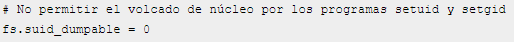
\includegraphics[width=13cm]{./Imagenes/2-C} 
	\end{center} 

{\bfseries fs.aio\_max\_nr}

\begin{center}
		
\includegraphics[width=5cm]{./Imagenes/3-C} 
	\end{center} 

 El kernel de Linux proporciona la función de E-S sin bloqueo asíncrono (AIO) que permite que un proceso inicie varias operaciones de E-S simultáneamente sin tener que esperar a que se complete ninguna de ellas. Esto ayuda a mejorar el rendimiento de las  aplicaciones que pueden solapar el procesamiento y la E-S.
El rendimiento puede ajustarse utilizando el -proc-sys-fs-aio-max-nrarchivo virtual en el sistema de archivos proc. El aio-max-nrparámetro determina el número máximo de solicitudes concurrentes permitidas.
Otro parámetro, -proc-sys-fs-aio-nrproporciona el número actual de solicitudes asíncronas en todo el sistema.
Veritas recomienda que establezca el aio-max-nrvalor en 1048576. Esto ayuda a HyperScale a tener un rendimiento óptimo, en un entorno que involucra grandes cargas de trabajo de E-S.

Realice los siguientes pasos en todos los nodos de cómputo y datos de HyperScale:
1.	Para establecer el aio-max-nrvalor, agregue la siguiente línea al -etc-sysctl.confarchivo:
 fs.aio-max-nr = 1048576
2.	Para activar la nueva configuración, ejecute el siguiente comando:
 -sysctl p etc-sysctl.conf
 
\newpage

{\bfseries fs.file-max}\\

Este es el máximo de descriptores de archivos (FD) implementado en un nivel de kernel, que no puede ser superado por todos los procesos sin aumentar. El ulimit se aplica en un nivel de proceso, que puede ser menor que el máximo de archivo. No hay riesgo de impacto en el rendimiento al aumentar el máximo de archivos. Las distribuciones modernas tienen el máximo establecido de FD bastante alto, mientras que en el pasado requería la re-compilación y modificación del kernel para aumentar más allá de 1024. \\ \\
No aumentaría en todo el sistema a menos que tenga una necesidad técnica. La configuración por proceso a menudo necesita ajustarse para servir a un demonio en particular, ya sea una base de datos o un servidor web. 
Si elimina el límite por completo, ese daemon podría agotar todos los recursos del sistema disponibles; lo que significa que no podrá solucionar el problema excepto si presiona el botón de reinicio o el ciclo de encendido. Por supuesto, es probable que cualquiera de ellos cause la corrupción de los archivos abiertos.
Establecer de forma persistente el límite de descriptores de fichero (/etc/sysctl.conf) a manejar del kernel.
	\begin{center}
		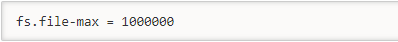
\includegraphics[width=8cm]{./Imagenes/fsFileE1} 
	\end{center}
Si se modifica el valor, se deben guardar los cambios y comprobar que el valor es el esperado.
	\begin{center}
		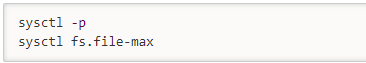
\includegraphics[width=8cm]{./Imagenes/fsFileE2} 
	\end{center}
Se puede consultar el valor en el fichero /proc/sys/fs/file-max y /proc/sys/fs/file-nr.
	\begin{center}
		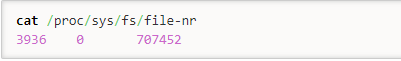
\includegraphics[width=8cm]{./Imagenes/fsFileE3} 
	\end{center}
El fichero file-nr muestra tres parámetros. 3936 Descriptores de ficheros asignados. 0 Descriptores de ficheros que no están en uso pero fueron asignados. 707452 Límite de descriptores de ficheros del sistema del sistema (/proc/sys/fs/file-max).\\ \\
{\bfseries kernel.shmmni}\\

Los parámetros SHMALL , shmmax y shmmni determinan cómo está disponible la cantidad de memoria compartida para Oracle para su uso. Estos parámetros se establecen en las páginas de memoria, no en bytes, por lo que los tamaños utilizables son el valor multiplicado por el tamaño de la página, típicamente 4096 bytes. Para confirmar el tamaño de página, utilice el comando -a getconf | grep PAGE\_SIZE
\begin{itemize}
	\item shmall : La cantidad total de memoria compartida (en páginas) que puede asignarse en el sistema de
	\item shmmax : El tamaño máximo de un segmento de memoria compartida (en páginas)
	\item shmmni : El número máximo de segmentos de memoria compartida disponible en el sistema
\end{itemize}
El valor para shmmni tiene que ser al menos tan alta como el número de bases de datos que están destinados a ser puesto en el sistema, pero en la práctica es generalmente mucho más alta (Oracle recomienda 4096.) \\ \\
La guía de instalación rápida incluye instrucciones sobre la comprobación de estos parámetros. Si necesitan ser modificados, se pueden establecer en el archivo /etc/sysctl.conf con las entradas como las siguientes:
	\begin{center}
	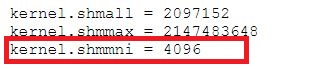
\includegraphics[width=8cm]{./Imagenes/kernelShimi} 
\end{center}

{\bfseries  kernel.sem}
\\
\\Los semáforos actúan como banderas para la memoria compartida. Los semáforos se activan o desactivan. Cuando un proceso de Oracle accede al SGA en la memoria compartida, busca un semáforo para esa porción de memoria. \\
\\
\\Los valores para los semáforos representan lo siguiente:\\
\\•	semmsl : el número de semáforos por conjunto
\\•	semmns : el número total de semáforos disponibles
\\•	semopm : el número de operaciones que se pueden realizar por llamada de semáforo
\\•	semmni : el número máximo de segmentos de memoria compartida disponibles en el sistema
\\

{\bfseries  net.ipv4.ip\_local\_port\_range}
\\
\\Define el rango de puertos locales que utilizan TCP y UDP para elegir el puerto local. El primer número es el primero, el segundo el último número de puerto local. \\
\\Si es posible, es mejor que estos números tengan una paridad diferente, es decir, uno par y uno impar. 
\\
	\begin{center}
		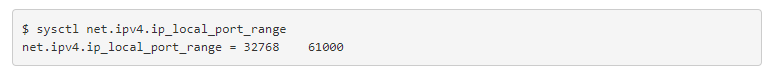
\includegraphics[width=17cm]{./Imagenes/c} 
	\end{center} 

{\bfseries  net.core.rmem\_default}
\\
\\Define el rango de puertos locales que utilizan TCP y UDP para elegir el puerto local. El primer número es el primero, el segundo el último número de puerto local. \\
\\Si es posible, es mejor que estos números tengan una paridad diferente, es decir, uno par y uno impar. 
\\
	\begin{center}
		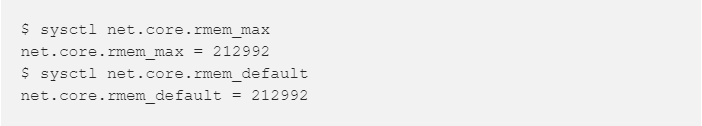
\includegraphics[width=17cm]{./Imagenes/t} 
	\end{center} 

{\bfseries  net.core.rmem\_max}
\\
\\Esto establece el tamaño máximo del búfer de recepción del sistema operativo para todos los tipos de conexiones.
\\
\\La configuración de net.core.rmem\_max define el tamaño máximo del búfer de socket de recepción en bytes.\\
\\
\\Hay algunas configuraciones diferentes que parecen ser muy similares. Puede ver que en Ubuntu 15.04 (3.18.0-13-generic) el valor predeterminado para net.core.rmem\_max es 212992. En este caso, los valores predeterminado y máximo son los mismos. Elevar este valor a un valor mayor aumentará el tamaño del búfer, pero esto puede tener efectos desagradables en términos de "acumulación de búfer". \\
	\begin{center}
		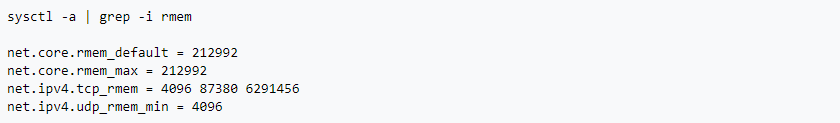
\includegraphics[width=17cm]{./Imagenes/s} 
	\end{center} 


{\bfseries  net.core.wmem\_default}
\\
\\Esto establece el tamaño del búfer de envío del sistema operativo predeterminado para todos los tipos de conexiones.
\\

{\bfseries  net.core.wmem\_max}
\\
\\Esto establece el tamaño del búfer de envío del sistema operativo predeterminado para todos los tipos de conexiones.
\\
\\La configuración de net.core.wmem\_max define el tamaño máximo del búfer de socket de envío en bytes.
\\
\\
Puede ver que en Ubuntu 15.04 (3.18.0-13-generic) el valor predeterminado para net.core.wmem\_max es 212992, que es del mismo tamaño que rmem\_max. Si aumenta esto a un valor mayor, aumentará el tamaño del búfer de envío.\\
\\
	\begin{center}
		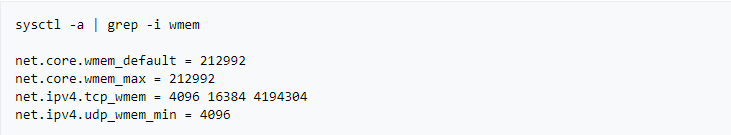
\includegraphics[width=17cm]{./Imagenes/p} 
	\end{center} 

5.2 ¿Con qué usuario(s) puedo conectarme al servidor a través del Administrador
Empresarial?
	\begin{center}
		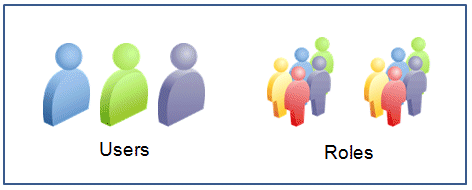
\includegraphics[width=13cm]{./Imagenes/users-oracle} 
	\end{center} 

	Los datos del login que se han utilizado para ingresar al Administrador Empresarial con:

	\begin{center}
		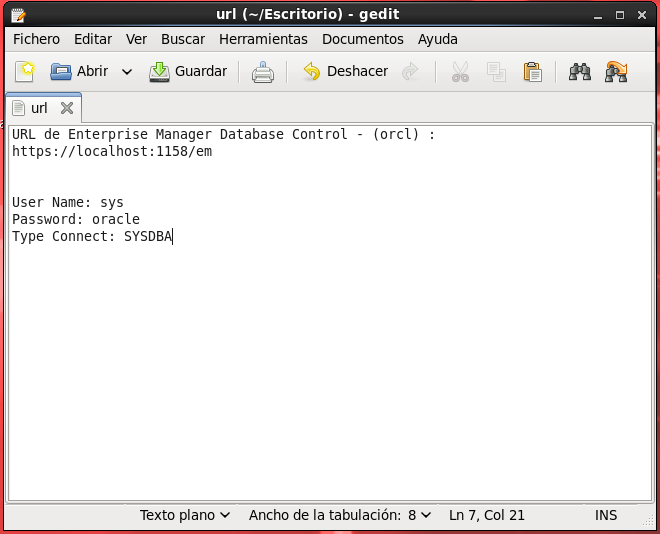
\includegraphics[width=15cm]{./Imagenes/94} 
	\end{center}

\vspace{\baselineskip}

5.3 Capture una imagen de pantalla del navegador con el Administrador Empresarial, con el nombre de su servidor e iniciada la sesión del usuario SYS.\\
\\
\\Para verificar de que la instalación ha sido exitosa, iniciar un navegador de Internet (Mozilla u otro similar), e introducir la dirección electrónica. Si todo es correcto aparecerá la interfaz de inicio de sesión de la herramienta Enterprise Manager (Administrador Empresarial) de Oracle.\\
\begin{center}
	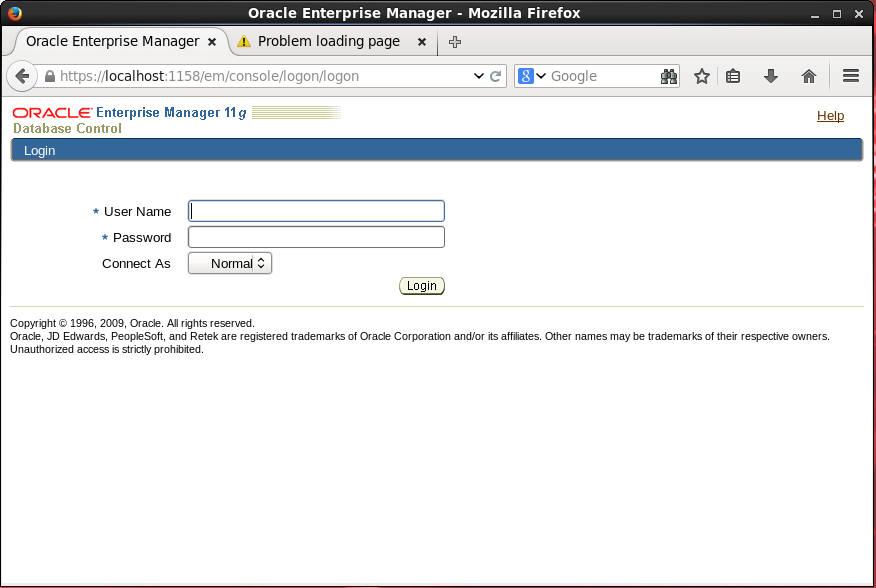
\includegraphics[width=16cm]{./Imagenes/91} 
\end{center}

Pero, si aparece la siguiente advertencia. para lo cual debemos ir a la Opcion I Understand the Risks
\begin{center}
	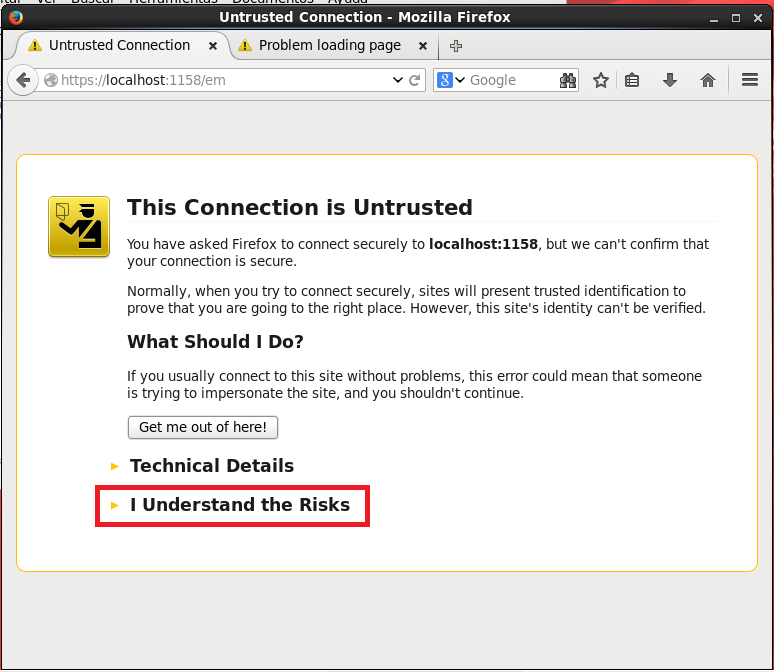
\includegraphics[width=15cm]{./Imagenes/88} 
\end{center}

Lo cual nos desglosara un comunicado, el cual presionamos el boton Add Exception
\begin{center}
	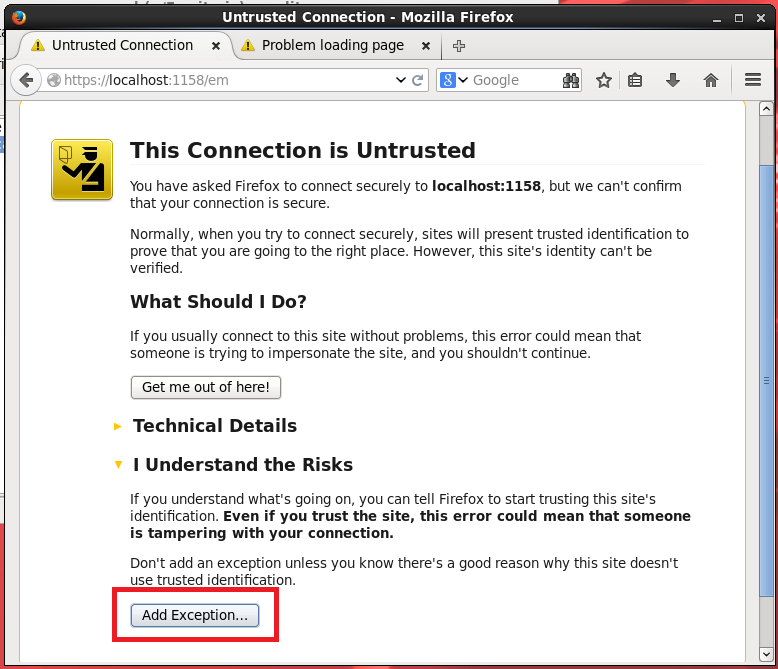
\includegraphics[width=15cm]{./Imagenes/89} 
\end{center}

Nos aparecera una nueva ventana de Advertencia donde presionaremos Confirm Security Exception
\begin{center}
	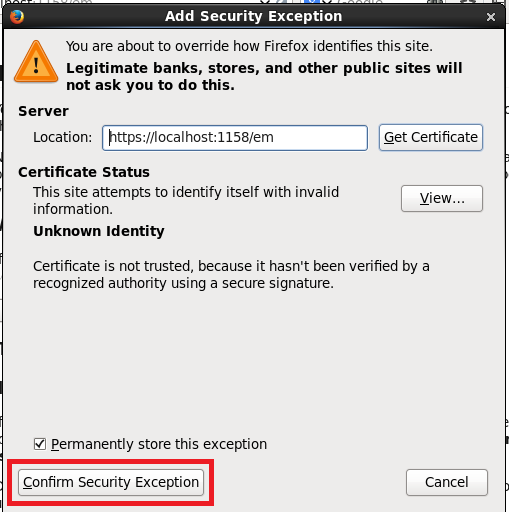
\includegraphics[width=10cm]{./Imagenes/90} 
\end{center}

Ya al culminar estos pasos podremos visualizar nuestra pagina de Login, donde podremos colocar nuestros datos
\begin{center}
	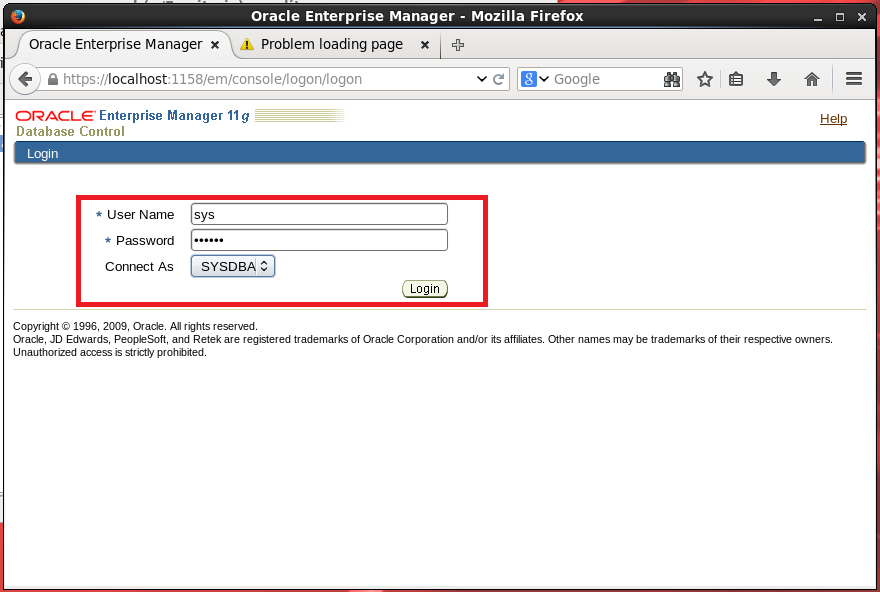
\includegraphics[width=15cm]{./Imagenes/92} 
\end{center}

Y cuando ingresemos nos aparecera la siguiente pagina de inicio
\begin{center}
	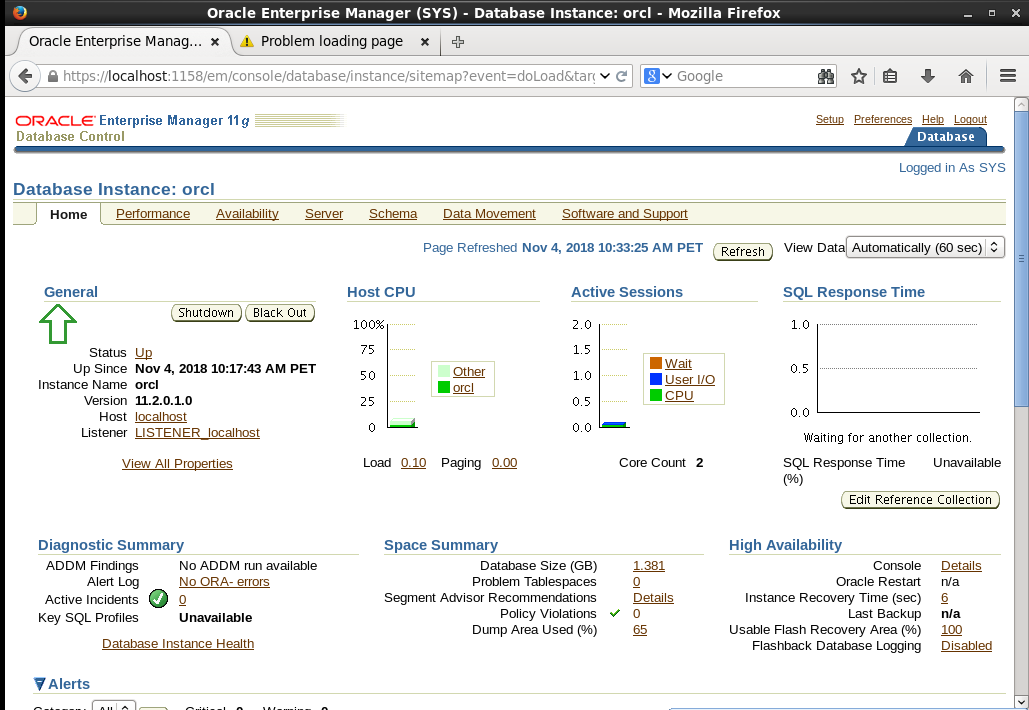
\includegraphics[width=15cm]{./Imagenes/93} 
\end{center}

Para no olvidarnos, es bueno mantener anotado la Url y los datos del Login.
\begin{center}
	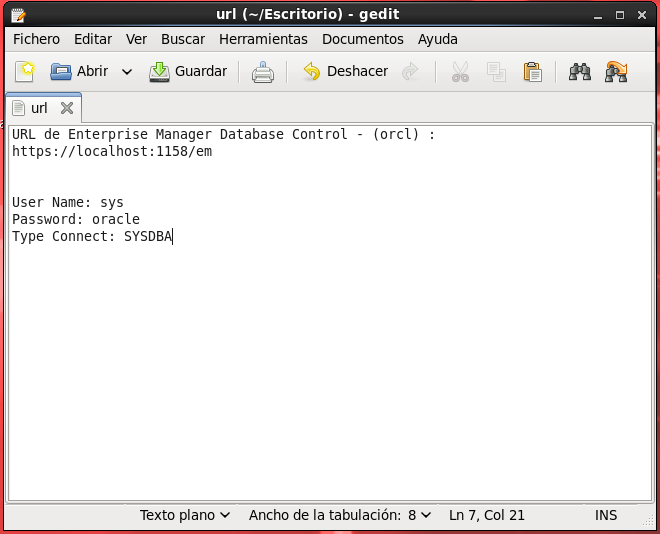
\includegraphics[width=15cm]{./Imagenes/94} 
\end{center}

